%TODO: more didactics (team work, ..)

% Make nice A4 pages for print:
%\usepackage{pgfpages}
%\pgfpagesuselayout{resize to}[a4paper,border shrink=5mm,landscape]

\beamertemplatenavigationsymbolsempty

\setbeamertemplate{bibliography item}[text]

\usepackage[type={CC},modifier={by-sa},version={4.0}]{doclicense}

\usepackage[utf8]{inputenc}
\usepackage{hyperref}
\usepackage{breakurl}
\usepackage{graphicx}
\usepackage{pgfplots}
\usepackage{pgf}
\usepackage{tikz}
\usetikzlibrary{positioning}
\usetikzlibrary{arrows}
\usetikzlibrary{decorations.markings}
\usetikzlibrary{calc}
\usetikzlibrary{matrix}
\usetikzlibrary{shapes}
\usetikzlibrary{decorations.pathmorphing}
\usetikzlibrary{fit}
\usetikzlibrary{backgrounds}
\usetikzlibrary{plotmarks}
\usepackage{stmaryrd}
\usepackage{listings}
\usepackage{pdflscape}
\usepackage{perpage}
\usepackage{appendixnumberbeamer}

%\usepackage[thmmarks,amsmath,amsthm]{ntheorem} % already included in beamer
\usepackage{thm-restate}

\usepackage[sort&compress,numbers]{natbib}  % to be have \citet, \citeauthor, \citeyear

\MakePerPage{footnote}

\tikzstyle{o}=[r,ppBlue]
\tikzstyle{r}=[thick,rectangle,align=center]
\tikzstyle{t}=[r,ppTrans] %,font=\bfseries]
\tikzstyle{dd}=[densely dashed]
\tikzstyle{n}=[r,ppBlue]
\tikzstyle{p}=[r,ppRed]
\tikzstyle{ppRed}  =[draw=red,  fill=  red!20]
\tikzstyle{ppBlue} =[draw=blue, fill= blue!20]
\tikzstyle{ppGreen}=[draw=green,fill=green!20]
\tikzstyle{ppTrans}=[draw=none, fill=none]

\usetheme{Warsaw}

\useoutertheme[subsection=true]{smoothbars}
%\useoutertheme[subsection=false]{miniframes}

\definecolor{bblue}{HTML}{D7DF01}	% yellow-ish actually, for better black/white printing
\definecolor{rred}{HTML}{C0504D}
\definecolor{ggreen}{HTML}{9BBB59}
\definecolor{ppurple}{HTML}{9F4C7C}
\definecolor{lightgray}{rgb}{0.3,0.3,0.3}
\definecolor{lightergray}{rgb}{0.9,0.9,0.9}
\definecolor{UniBlue}{RGB}{83,121,170}

\DeclareTextFontCommand\textintro{\normalfont\bfseries\itshape} % nice!
\newcommand{\intro}[2][]
{%
	\textintro{#2}%
}
\newcommand{\empha}[2][]
{%
	\emph{#2}%
}

%\theoremstyle{plain}
\newcounter{reqcounter}
\newtheorem{requirement}[reqcounter]{Requirement}

%setbeamercolor{structure}{fg=violet}

\makeatletter
\def\th@task{%
    \normalfont % body font
    \setbeamercolor{block title example}{bg=orange,fg=white}
    \setbeamercolor{block body example}{bg=orange!20,fg=black}
    \def\inserttheoremblockenv{exampleblock}
  }
\makeatother

\theoremstyle{task}
\newtheorem{task}{Task}

\newenvironment{assignment}%
{%\setbeamercolor{background canvas}{bg=violet}%
%\setbeamercolor{structure}{fg=cyan!90!black}%
 \setbeamercolor{frametitle}{bg=orange,fg=white}
\begin{frame}}%
{\end{frame}}%

\AtBeginSection[]{
  \begin{frame}
  \vfill
  \centering
  \begin{beamercolorbox}[sep=8pt,center,shadow=true,rounded=true]{title}
    \usebeamerfont{title}\insertsectionhead\par%
  \end{beamercolorbox}
  \tableofcontents
  \vfill
  \end{frame}
}




\pgfplotsset{compat=1.14}
\author{Markus Raab}


\date{12.06.2019}

\begin{document}

\renewcommand{\enquote}[1]{\emph{``#1''}} % Cannot be done earlier

%%%%%%%%%%%%%%%%%%%%%%%%%%%%%%%
\begin{frame}
	\titlepage
	\doclicenseThis
\end{frame}

\begin{frame}
	Lecture is every week Wednesday 09:00 - 11:00.

	\begin{description}
		\item[06.03.2019:] {\color{gray}topic, teams}
		\item[13.03.2019:] {\color{gray}TISS registration, initial PR}
		\item[20.03.2019:] {\color{gray}other registrations, guest lecture}
		\item[27.03.2019:] {\color{gray}PR for first issue done, second started}
		\item[03.04.2019:] {\color{gray}first issue done, PR for second}
		\item[10.04.2019:] {\color{gray}mid-term submission of exercises}
		\item[08.05.2019:] {\color{gray}different location: Complang Libary}
		\item[15.05.2019:]
		\item[22.05.2019:] {\color{gray}all 5 issues done}
		\item[29.05.2019:]
		\item[05.06.2019:] {\color{gray}final submission of exercises}
		\item[12.06.2019:]
		\item[19.06.2019:] last corrections of exercises and register for exam
		\item[26.06.2019:] exam
	\end{description}
\end{frame}

\begin{assignment}
	\frametitle{Tasks}

	\begin{task}
	\begin{itemize}[<+-| alert@+>]
	\item personal feedback about me in TISS Stimmungszettel (anonym) or by email (markus.raab@complang.tuwien.ac.at).
	\end{itemize}
	\end{task}
\end{assignment}

\begin{frame}
	\frametitle{Popular Topics}
	\vspace{-0.55cm}
	\setlength{\columnsep}{-1.3cm}
	\raggedright
	\definecolor{amethyst}{rgb}{0.6, 0.4, 0.8}
	\begin{multicols}{2}
	\begin{description}
	\item[14] {\color{red} tools}
	\item[9] {\color{gray} testability}
	\item[9] {\color{gray} code-generation}
	\item[7] {\color{gray} context-awareness}
	\item[6] {\color{red} specification}
	\item[6] {\color{gray} misconfiguration}
	\item[6] {\color{gray} complexity reduction}
	\item[5] {\color{amethyst} validation}
	\item[5] {\color{gray} points in time} % (early detection)
	\item[5] {\color{red} error messages}
	\item[5] {\color{gray} auto-detection}
	\item[4] {\color{red} user interface}
	\item[4] {\color{gray} introspection}
	\item[4] {\color{gray} design}
	\item[4] {\color{gray} cascading}
	\item[4] {\color{gray} architecture of access}
	\item[3] {\color{gray} configuration sources}
	\item[3] {\color{gray} config-less systems}
	\item[2] secure conf
	\item[2] {\color{gray} architectural decisions}
	\item[1] {\color{amethyst} push vs.\ pull}
	\item[1] {\color{amethyst} infrastructure as code}
	\item[1] {\color{red} full vs.\ partial}
	\item[1] convention over conf %iguration
	\item[1] CI/CD
	\item[0] {\color{gray} documentation}
	\end{description}
	\end{multicols}
\end{frame}

\begin{frame}
	\frametitle{Learning Outcomes}
	Students will be able to
	\begin{itemize}
	\item connect needs of CM tools with configuration specifications.
	\item remember differences between CM languages.
	\item contextualize CM languages with the view point of administrators.
	\end{itemize}
\end{frame}


%%%%%%%%%%%%%%%%%%%%%%%%%%%%%%%%%%%%%%%%%% 
\section{Recapitulation}

\subsection{}

\begin{frame}
	\frametitle{Types of Specifications (Recapitulation)}

	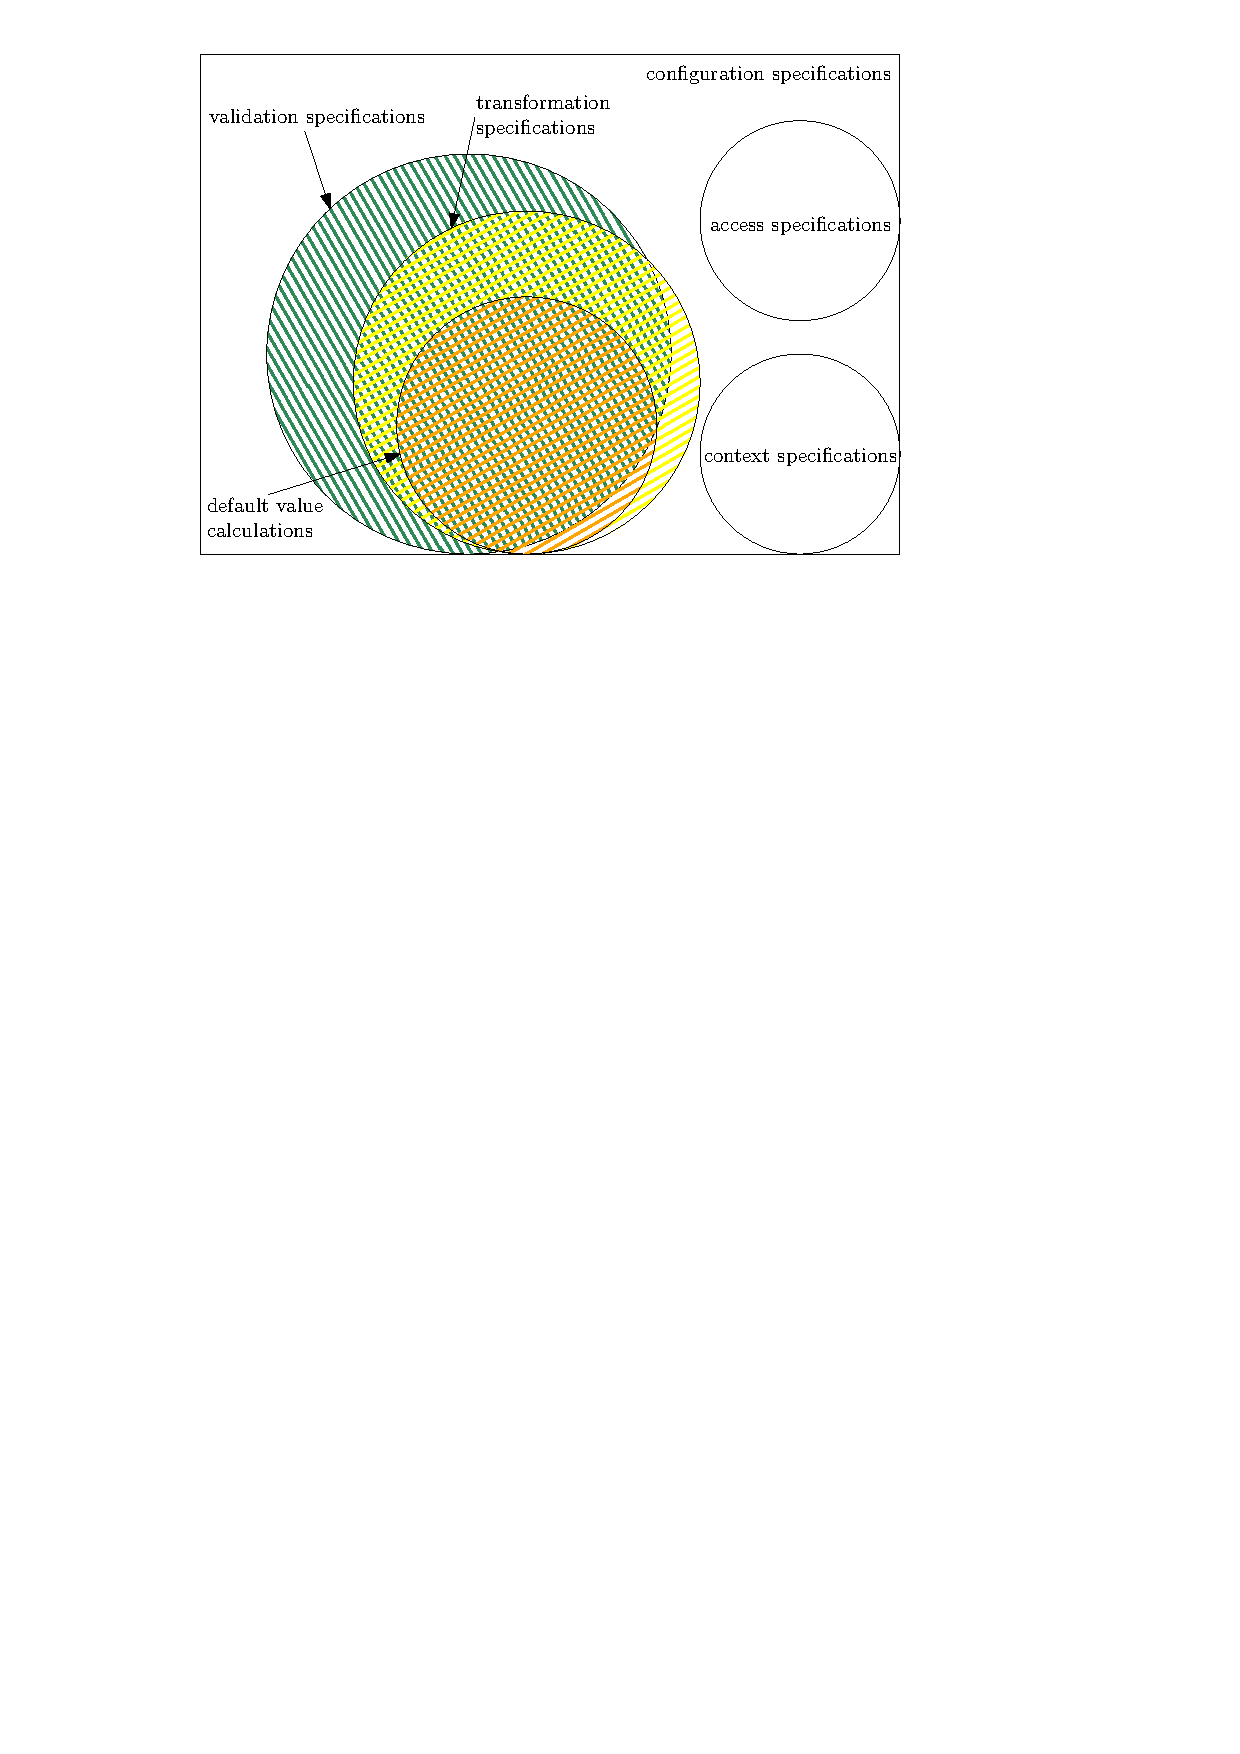
\includegraphics[scale=0.8]{specifications}
\end{frame}


\begin{frame}
	\frametitle{Configuration Specification (Partly Recapitulation)}

	\begin{task}
	How can we combine configuration specifications and configuration management?
	(Think, Pair, Share)
	\end{task}

	\pause

	\begin{itemize}[<+-| alert@+>]
	\item Configuration settings are an instantiation of the configuration specifications. \\
		Code describing the instantiation is \textbf{CM code}.
	\item Configuration design is explicit (like transformations and default values) and can help while writing CM code.
	\item CM code can even be generated from the specification.
	\item Access specifications make access trivial via uniform interface.
	\item Visibility and similar techniques may help dealing with complexity.
	\end{itemize}
\end{frame}

\begin{frame}
	\frametitle{Configuration Drift (Recapitulation)}

	\begin{task}
	What is configuration drift? What are its causes?
	\end{task}

	\pause

	Are derivations of the ``Single Source of Truth'' (the CM code).

	Caused by:

	\begin{itemize} %[<+-| alert@+>]
	\item manual configuration changes by administrators
	\item manual configuration changes by end users
	\item differences in updates (e.g., skipped or failed updates)
	\item failed attempts to change configuration
	\item applying different versions of CM code
	\item \dots
	\end{itemize}


\end{frame}

\begin{frame}
	\frametitle{Push vs.\ Pull (Recapitulation)}

	\begin{task}
	Explain the Push and the Pull Model.
	What are their (dis)advantages?
	\end{task}

	\pause

	\begin{itemize} %[<+-| alert@+>]
	\item Push is more interactive.
	\item Push cannot do its job if nodes are not reachable.
	\item Push needs additional techniques to scale with many nodes.
	\item Push demands access to servers from a single server.
	\item Pull needs additional monitoring to know when a patch has been applied.
	\item Pull needs resources even if nothing is to do.
	\end{itemize}
\end{frame}


\begin{frame}
	\frametitle{Properties (Recapitulation)}

	\begin{task}
	What is idempotent, self-describing, round-tripping configuration?
	\end{task}

	\pause


	\begin{description}
	\item[Idempotent]
	yield the same configuration with any number of applications from CM code ($n\ge1$)~\cite{waldemar2013testing}:
	\[
		f(f(x))=f(x)
	\]
	needed to guarantee repeatability

	\item[Self-describing]
	means that from the configuration file alone we are able to derive the correct data structure~\cite{wadler2003xml}.

	\item[Round-tripping]
	means that if a data structure is serialized and then parsed again, we end up with an identical data structure~\cite{wadler2003xml}.
	\end{description}

	The data structure could be a KeySet.
\end{frame}

\begin{frame}
	\frametitle{Examples}

	XML has neither of the last two properties~\citet{wadler2003xml}:

	\begin{itemize}[<+-| alert@+>]
	\item internal representation crucially depends on XML schema
	\item union of integer and strings
	\end{itemize}

	\pause[\thebeamerpauses]  %  show after \begin{itemize}[<+->]

	\citet{waldemar2013testing} tested 298 Chef scripts, of which 92 were non-idempotent:

	\begin{itemize}[<+-| alert@+>]
	\item \texttt{/etc/timezone} rewritten by package tzdata
	\item tomcat6: files copied by user if \texttt{/etc/tomcat6/tomcat6.conf} does not exist but copy fails because later step creates \texttt{/etc/tomcat6/logging.properties} as root.
	\item mongodb: if installation fails, the group ``mongodb'' does not exist, failing at later tasks creating directories using this group
	\end{itemize}
\end{frame}

\begin{frame}
	\frametitle{Checking Configurations (Recapitulation)}

	\begin{task}
	Which properties of configuration settings can be checked?
	\end{task}

	\pause

	\begin{itemize} %[<+-| alert@+>]
	\item structure
	\item values (data types)
	\item constraints
	\item semantic checks (e.g., IP, folder)
	\item domain-specific checks (e.g., databases)
	\item requirements (suitable configurations)
	\item context (context-aware configurations)
	\end{itemize}
\end{frame}

\begin{frame}
	\frametitle{Checking Specifications (Recapitulation)}

	\begin{task}
	What are the goals of checking \elektra{Spec}?
	\end{task}

	\pause

	\begin{itemize} %[<+-| alert@+>]
	\item Defaults must be present for safe lookups.
	This goal also implies that there must be at least one valid configuration setting.
	\item Types of default values must be compatible with the types of the keys.
	\item Every contextual interpretation of a key must yield a compatible type.
	\item Links must not refer to each other in cycles.
	\item Every link and the pointee must have compatible types.
	\end{itemize}
\end{frame}

%%%%%%%%%%%%%%%%%%%%%%%%%%%%%%%%%%%%%%%%%% 
\section{CM languages}

\subsection{}

\begin{frame}[fragile]
	\frametitle{Proteus (PCL)}
	\textsc{Proteus}~\cite{tryggeseth1995modelling} shows the tight relation between software configuration management, like Git or Svn, and configuration specification languages.
	\textsc{Proteus} (PCL) combines both worlds in a powerful build system.

	\begin{code}[basicstyle=\tiny,morekeywords={family,attributes,end,physical,default,classifications},gobble=4,language=]
	family CalcProg
		attributes
			HOME : string default "/home/ask/proteus/test";
			workspace := HOME ++ "/calc/src/"; // string concatenation
			repository := "calc/";
			end
		physical
			main => "main.C";
			defs => "defs.h";
			exe => "calc.x" attributes workspace := HOME ++ "/calc/bin"; end
			classifications status := standard.derived; end;
		end
	end
	\end{code}
\end{frame}

\begin{frame}
	\frametitle{NIX}

	The NIX language~\cite{dolstra2007purely} claims to be purely functional as a novel feature.
	The main concept is the referential transparency both for the configuration specification language and for the system itself.

	\textbf{Expressiveness:}
	NIX expressions, for example functions, describe how to build software packages.

	\textbf{Reasoning:}
	Because of the referential transparency of the system itself, every solution derived from the NIX expressions should be valid, so no reasoning or conflict handling is necessary.

	\textbf{Modularity:}
	The NIX expressions are modular because they ensure absence of side effects and thus can be easily composed.

	\textbf{Reusability:}
	Derivations that describe atomic build actions are reused in other derivations.
\end{frame}

\begin{frame}
	\frametitle{UML}
	\citet{felfernig1999knowledge,felfernig2000uml,felfernig2002joint} describe an approach where the unified modeling language (UML) is used as notation.

	\textbf{Expressiveness:}
	All UML features, including cardinality, domain-specific stereotypes and OCL-constraints are available.
	The basic structure of the system is specified using classes, generalization and aggregation.

	\textbf{Reasoning:}
	Customers provide additional input data and requirements for the actual variant of the product.

	\textbf{Modularity:}
	Generalization is present without multiple inheritance with disjunctive semantics, i.\,e., only one of the given subtypes will be instantiated.

	\textbf{Reusability:}
	For shared aggregation additional ports are defined for a part.
\end{frame}


\begin{frame}
	\frametitle{CFEngine}

	CFEngine~\cite{burgess2003theory,burgess1995cfengine,pandey2012investigating} is a language-based system administration tool that pioneered idempotent behavior.

	\textbf{Expressiveness:}
	CFEngine allows us to declare dependences and facilitates some high-level configuration specification constructs.
	In its initial variants it neither had validation specifications, cardinalities, nor higher-level relationships.

	\textbf{Reasoning:}
	Not supported.

	\textbf{Modularity:}
	Not supported.

	\textbf{Reusability:}
	Existing system administrator scripts can be profitably run from CFEngine.
\end{frame}



\begin{frame}
	\frametitle{Quattor (Pan)}

	\citet{cons2002pan} invented and used PAN for many machines within CERN.

	\textbf{Expressiveness:}
	The Pan language allows users to specify data types, validation with code snippets and constraints.
	The compiler uses a 5 step process: compilation, execution, insertions-of-defaults, validation, and serialization.

	\textbf{Reasoning:}
	Pan focuses on validating configurations, it is not able to generate new configurations.
	Pan provides type enforcement with embedded validation code.

	\textbf{Modularity:}
	The language has user-defined data types (called templates) but otherwise has only minimal support for modularity.

	\textbf{Reusability:}
	Reusability and collaboration is only possible via simple include statements and a simple inheritance mechanism of templates.
\end{frame}


\begin{frame}
	\frametitle{ConfValley (CPL)}

	\citet{huang2015confvalley} introduce systematic validation for cloud services.
	ConfValley uses a unified configuration settings representation for tens of different configuration file formats.

	\textbf{Expressiveness:}
	CPL is not able to specify dynamic and complex requirements.

	\textbf{Reasoning:}
	Constraints can be inferred by running an inference engine on configuration settings that are considered good (black-box approach).
	Within the validation engine, however, no constraint solver is available.

	\textbf{Modularity:}
	CPL aims at easy grouping of constraints.
	Adding language primitives need modifications in the compiler.

	\textbf{Reusability:}
	Using transformations and compositions, predicates can be reused in different contexts.
	Also with language constructs like \texttt{let}, specifications can be reused.
\end{frame}

\begin{frame}
	\frametitle{Popular CMs today}

	\begin{itemize}[<+-| alert@+>]
	\item CFengine (1993)
	\item LCFG (1994)
	\item Quattor (2005)
	\item Puppet (2005)
	\item Chef (2009)
	\item Salt (2011)
	\item Ansible (2012)
	\item Mgmt (2016)
	% TODO: something new?
	\end{itemize}
\end{frame}



%%%%%%%%%%%%%%%%%%%%%%%%%%%%%%%%%%%%%%%%%% 
\section{Error Messages}

\subsection{}

\begin{frame}[fragile]
	\frametitle{Motivation (Recapitulation)}

	Error messages are extremely important as they are the main communication channel to system administrators.\\
	\vspace{0.5em}

	\begin{code}[morekeywords={assign,math},gobble=4]
	[a]
	  check/type:=long
	[b]
	  check/type:=long
	[c]
	  check/range:=0-10
	  assign/math:=../a+../b
	\end{code}

	\begin{task}
	Where should the error message point to if we change b to 10 \\ (a is unchanged 1)?
	\end{task}
\end{frame}

\begin{frame}
	\frametitle{Considerations (Recapitulation)}

	\begin{task}
	What needs to be considered when designing error messages?
	\end{task}

	\begin{itemize} %[<+-| alert@+>]
	\item Generic vs.\ specific plugins
	\item Precisely locate the cause (and do not report aftereffects)
	\item Give context
	\item Personification~\cite{lee2011personifying}
	\end{itemize}
\end{frame}

\begin{frame}
	\frametitle{Further Considerations}

	\begin{itemize}[<+-| alert@+>]
	\item configuration design first: avoid errors if possible
	\item ``edit here mentality'': do not point to correct statements~\cite{marceau2011mind}
	\item precision and recall\footnote{terms from classification, it is the numerical counterpart of soundness and completeness}~\cite{wrenn2017error}
	\item error messages should not leak internals~\cite{brown1983error}
	\item do not propose solutions~\cite{marceau2011mind} if you are not sure
	\item reduce vocabulary~\cite{marceau2011mind}
	\item tension between providing enough information and not overwhelming the user~\cite{wrenn2017error}
	\item colors might help~\cite{wrenn2017error}
	\end{itemize}
\end{frame}

\begin{frame}
	\frametitle{Error Messages for Misconfiguration~\cite{zhang2015proactive}}

	\begin{itemize}[<+-| alert@+>]
	\item error messages are often the sole data source
	\item tool uses misconfiguration injection and checks if error message point to the correct setting
	\item tool requires system tests
	\item they considered error message as okay if key \emph{or} value is present
	\end{itemize}

	\pause[\thebeamerpauses]  %  show after \begin{itemize}[<+->]

	\begin{alertblock}{Implication}
	Missing error message means the configuration specification is not complete.
	\end{alertblock}
\end{frame}

\begin{frame}
	\frametitle{Context for error messages}

	Error messages should contain:

	\begin{itemize}[<+-| alert@+>]
	\item pin-point key (which also pin-points to the specification)
	\item repeat relevant parts of values and the specification
	\item show mountpoint (to make relative keys unique)
	\item show file name and line number
	\item for reporting bugs: show source code lines
	\end{itemize}
\end{frame}

\begin{frame}[fragile]
	\frametitle{Precise Location (Recapitulation)}

	\begin{code}[language=CfgElektra,gobble=4]
	a=5  ; unmodified
	b=10 ; modification bit in metadata
	     ; is only set here
	c=15 ; unmodified by user but changed
	     ; later by assign/math
	\end{code}
\end{frame}

\begin{frame}[fragile]
	\frametitle{Example Error Messages (Recapitulation)}
\begin{verbatim}
Sorry, I was unable to change the configuration settings!
Description: I tried to set a value outside the range!
Reason: I tried to modify b to be 10 but this caused c to
        be outside of the allowed range (0-10).
Module: range
At: sourcefile.c:1234
Mountpoint: /test
Configfile: /etc/testfile.conf
\end{verbatim}
\end{frame}

\begin{frame}[fragile]
	\frametitle{Example Error Messages (Improvement)}
\begin{verbatim}
Sorry, module range issued error C03100:
I tried to modify b to be 10 but this caused c to
be outside of the allowed range (0-10).
\end{verbatim}
\end{frame}




%%%%%%%%%%%%%%%%%%%%%%%%%%%%%%%%%%%%%%%%%% 
\section{User View}

\subsection{}

\begin{frame}
	\frametitle{User View}

	Who is the user of CM?

	\begin{itemize}[<+-| alert@+>]
	\item End Users?
	\item Developers (devs)?
	\item System Administrators (admins)?
	\end{itemize}
\end{frame}

\begin{frame}
	\frametitle{System Administrator Research}

	\begin{itemize}[<+-| alert@+>]
	\item Interest of understanding administrators emerged around 2002~\cite{anderson2002researching}.
	\item Typical methods are surveys, diary studies, interviews and observations (ethnographic field studies).
	\item Field studies also done in industry \cite{barrett2004field}.
	\item Barrett \cite{barrett2003system} tried to initiate a workshop at CHI 2003 to draw the attention of the HCI community towards system administration.
	\item The workshop was already dropped in the next year.
	\item The tenor is that ``tools ... are not well aligned''~\cite{haber2007design}.
	\item Research mainly looks at pre-CM. Manual administration is still standard (Source: e.g., Luke Kanies).
	\end{itemize}
\end{frame}


\begin{frame}
	\frametitle{CM research}

	In the meanwhile at Large Installation System Administrator Conference (LISA):

	\begin{itemize}[<+-| alert@+>]
	\item began as CFengine Workshop at LISA 2001
	\item CM workshop by Paul Anderson~\cite{anderson2002researching}
	\item in LISA 2003 an informal poll asked about CM tools: \\
	 	the only user of each tool in the room at the time was its author~\cite{burgess2006modeling}
	\item it is easy to invent CM tools (and configuration file formats)
	\item it is difficult to make it useful beyond your own goals
	\end{itemize}
\end{frame}

\begin{frame}
	\frametitle{Tasks}

	What do system administrators do?

	\begin{itemize}[<+-| alert@+>]
	\item keep our infrastructure running
	\item coordinate
	\item do backups
	\item manage hardware
	\item do inventory
	\item install applications
	\item manage security
	\item configure applications
	\item troubleshoot
	\item $\implies$ the unsung heroes!
	\end{itemize}
\end{frame}


\begin{frame}
	\frametitle{7 people, 1 command-line~\cite{barrett2004field}}

	\begin{itemize}[<+-| alert@+>]
	\item system administrator misunderstood problem \\ (had a wrong assumption)
	\item 7 people sought attention and trust, competing to tell the admin what to do
	\item due to wrong assumption the admin communicated to everyone, people could not help
	\item there were several instances in which the admin ignored or misinterpreted evidence of the real problem
	\item eventually someone else solved the problem: admin confused ``from''/``to'' port in the settings and firewall blocked requests
	\end{itemize}
\end{frame}

\begin{frame}
	\frametitle{other cases~\cite{barrett2004field}}

	\begin{itemize}[<+-| alert@+>]
	\item lost semicolon: execution of script failed due to missing semicolon, then they tried to delete a non-existent table.
	\item crontab: onltape/ofltape confused because of discussion about offline backup (although an online backup should be performed).
	\item crit sit: many system administrators competed against each other trying to write a simple script. The crit sit continued for two weeks.
	\end{itemize}
\end{frame}


\begin{frame}
	\frametitle{\citet{haber2007design}}

	Later \citet{haber2007design} repeated an ethnographic field study.
	The stories are similar to \citet{barrett2004field}.
	Their study was also conducted in the same company.
	They created personas:

	\begin{itemize}
	\item database administrator
	\item web administrator
	\item security administrator
	\end{itemize}
\end{frame}



\begin{frame}
	\frametitle{Database Administrator~\cite{haber2007design}}

	\begin{itemize}[<+-| alert@+>]
	\item frequent contact via phone, e-mail and IM
	\item needs to work on weekends
	\item pair-programming for new tasks
	\item typical errors: stopping wrong database process
	\end{itemize}
\end{frame}

\begin{frame}
	\frametitle{Web Administrator~\cite{haber2007design}}

	\begin{itemize}[<+-| alert@+>]
	\item crit sit
	\item deploying new Web applications
	\item about 20-400 steps to deploy an application
	\item moving from test to production done by hand
	\end{itemize}
\end{frame}

\begin{frame}
	\frametitle{Security Administrator~\cite{haber2007design}}

	\begin{itemize}[<+-| alert@+>]
	\item gets emails on suspicious activities
	\item multi-user chat
	\item ad-hoc scripts
	\end{itemize}
\end{frame}


\begin{frame}
	\frametitle{\citet{haber2007design}}

	\begin{itemize}[<+-| alert@+>]
	\item ``if data is lost...that is when you write your résumé.''
	\item \p{90} is spent with communicating with other admins
	\item only \p{6} is gathering information and running commands
	\item quality control: monitoring found that non-functional service was down two days
	\end{itemize}
\end{frame}


\begin{frame}
	\frametitle{\citet{barrett2004field}}

	\begin{itemize}[<+-| alert@+>]
	\item \p{20} of the time is spent in diversions
	\item \p{20} of the time people communicated about \emph{how to communicate}
	\item CLIs were generally preferred
	\item configuration and log files are scattered, poorly organized and often used inconsistent terminology
	\end{itemize}
\end{frame}


\begin{frame}
	\frametitle{Findings \cite{barrett2004field}}

	\begin{itemize}[<+-| alert@+>]
	\item syntax checking is essential
	\item replicating actions (e.g., to production) is error-prone
	\item undo not available
	\item do not assume a complete mental model (``if understand the system is a prerequisite [...], we are lost'')
	\item do not assume programming skills (only \p{35} reported having a bachelor's degree)
	\item trust in CLI tools but little trust in GUIs (is the information up-to-date?)
	\item errors while executing scripts lead to inconsistent state, rerunning often does not work
	\item[] (not idempotent)
	\end{itemize}
\end{frame}

\begin{frame}
	\frametitle{Design Principles \cite{haber2007design}}

	Many design principles for tools were given~\cite{haber2007design}:

	\begin{itemize}[<+-| alert@+>]
	\item configuration and logs should be displayed in a uniform way
	\item APIs/plugins for tools should be provided
	\item errors in configuration need to be discovered quickly
	\item confusion of similar settings should be avoided
	\item provide means of comparing configuration settings
	\item provide consistent profiles of information
	\item both transient and persistent settings should be visible
	\item when errors occur: always display which changes have been made (modern approach is idempotence)
	\end{itemize}
\end{frame}

\begin{frame}
	\frametitle{Apply to CM}

	What can we learn from manual system administration?

	\setbeamersize{description width=1cm}
	\begin{description}[<+-| alert@+>]
	\item[$+$] intensive review process catches errors
	\item[$-$] collaboration ineffective
	\item[$-$] context/situational awareness is essential
	\item[$+$] precise editing of configuration files works well
	\item[$+$] self-written tools are very efficient
	\end{description}

	\pause[\thebeamerpauses]  %  show after \begin{itemize}[<+->]

	\begin{alertblock}{Idea}
	Replicate parts that work well, automate error-prone parts.
	\end{alertblock}
\end{frame}

\begin{frame}
	\frametitle{Precise Editing}

	Partial modifications (precise editing) is natural for humans. \\
	It ensures preservations of (potentially security-relevant!) defaults. \\
	In CM following methods are used:

	\begin{itemize}[<+-| alert@+>]
	\item embed shell commands to do the work
	\item replace full content of configuration files
	\item replace full content of configuration files with templates
	\item line based manipulation (e.g., file\_line): match line and replace it
	\item Augeas/XML: match a key with XPath and replace it
	\item Elektra: set the value of a key
	\end{itemize}
\end{frame}

\begin{frame}
	\frametitle{Apply to CM}

	Elektra's goals are:

	\begin{itemize}[<+-| alert@+>]
	\item it should be easy to develop new high-level tools
	\item precise editing: change the configuration value as specified
	\end{itemize}

	\pause[\thebeamerpauses]  %  show after \begin{itemize}[<+->]

	Administrators/Devs still need to:

	\begin{itemize}[<+-| alert@+>]
	\item intensively review and improve the specifications
	\item test (and debug) configuration settings
	\end{itemize}

	\pause[\thebeamerpauses]  %  show after \begin{itemize}[<+->]

	Open topics (incomplete):

	\begin{itemize}[<+-| alert@+>]
	\item safe migrations of settings and data
	\item collaboration
	\item management (including knowledge)
	\end{itemize}
\end{frame}

\begin{frame}
	\frametitle{Conclusion}

	\begin{itemize}[<+-| alert@+>]
	\item Configuration management languages differ widely.
	\item Configuration specifications are helpful in different ways.
	\item Do not design around tools but design tools around you.
	\item Outlook: Go more in-depth into CM languages, contextualize with our topics
	\end{itemize}
\end{frame}



%%%%%%%%%%%%%%%%%%%%%%%%%%%%%%%%%%%%%%%%%% 
\nocite{raab2017introducing}

\appendix

\begin{frame}[allowframebreaks]
	\bibliographystyle{plainnat}
	\bibliography{../shared/elektra.bib}
\end{frame}

\end{document}


%TODO: add cliffhanger with preview for next time
